
%----------------------------------------------------------------------------------------
%	Lecture 1
%----------------------------------------------------------------------------------------

\chapter{Direction Fields and Integral Curves}  

\bigbreak
\section{First Order ODEs}

First Order ODEs are in the form $y' = f(x, y)$.

Examples : \ilds{y' = \frac{x}{y}}, $y ' = x - y^2$ and $y' = y - x^2$.

You can solve the first one just by separating the variables as $y dy = x dx$.
The second and third look very similar but the third one is easily solvable.
The second one is unsolvable, that is, there are no elementary functions which satisfy this equation.

Most eqautions are unsolvable. We will spend today on numerical and geomtric methods to solve the differential equations.

\section{Geometric View of Differential Equations}

Analytically, if $y' = f(x, y)$ and $y_1(x)$ is one of the solutions to this equation.

Geometrically, the differential equation correspond to a Direction Field.
And the solution corresponds to an Integral Curve.

A Diretion Field is field of a line element at each point in the $XY$-plane with slope $f(x, y)$.
Now we fill all the plane with these lines.

An Integral Curve is a curve that is tangent to the line element of every point that it passes.
That is at all points on the curve the tangent line has the direction same as the Direction Field.

\begin{figure}[ht!]
    \centering
    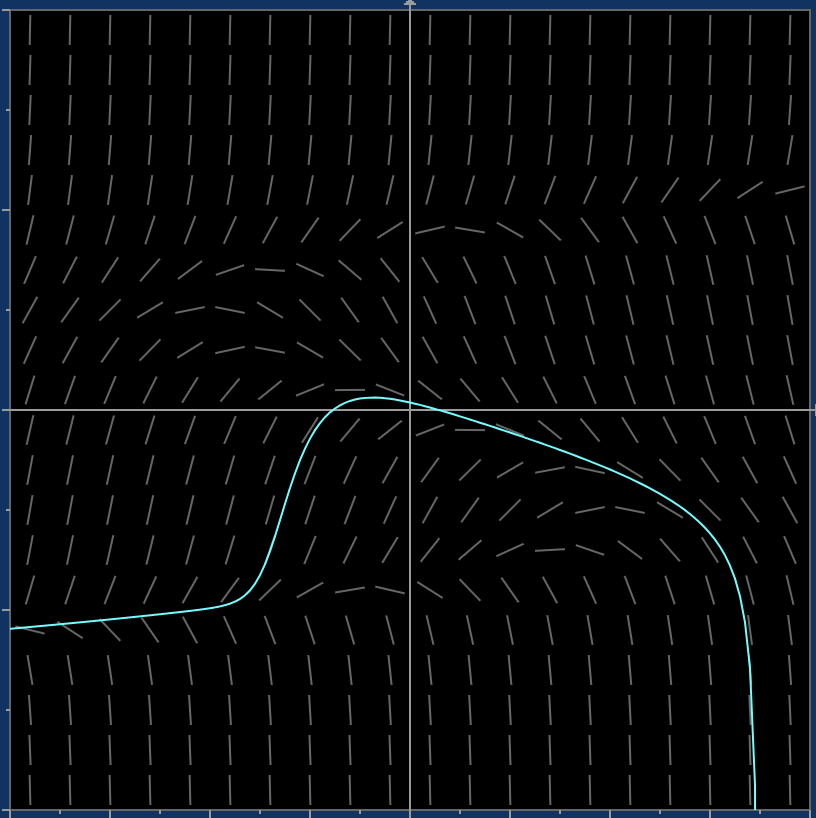
\includegraphics[scale=0.5]{./images/lecture_1_figure_1.png}
    \caption{Direction Field and Integral Curves}
\end{figure}

{\bf Theorem : } Given $y_1(x)$ is a solution to the equation of $y' = f(x, y)$
iff the graph of $y_1(x)$ is an Integral Curve of the Direction Field of the equation $y' = f(x, y)$.

{\bf Proof : } 
To prove this we can just evaluate both sides. That is, $y_1(x)$ is a solution to $y' = f(x, y)$ 
then $y_1'(x) = f(x, y_1'(x))$ at every point. 
That is at every point of the curve, the slope of the curve is the same as $f(x, y)$.

The Integral Curve of a direction field means that at every point of the curve is equal to $f(x, y)$.

Thus, both these reduce to the same statement. Hence, Proved.

\subsection{Drawing a Direction Field}

For computers, pick equally spaced points and calculate the slope at each point.
Then put line elements at each of those points.

For humans, calculating $f(x, y)$ at every point is tedious.
So 
\begin{enumerate}
    \item Pick a slope $c$.
    \item Plot the equation $f(x, y) = c$.
    \item This curve is called Isocline.
\end{enumerate}

Here, we draw a curve where the slope $c$ at every point. 
So then you can draw line elements with slope $c$ at every point.


{\bf Example : } Let \ilds{y' = \frac{-x}{y}}

Here, the equation for Isoclines will be \ilds{\frac{-x}{y} = c \Rightarrow y = -\frac{x}{c}}
Here the Isoclines will be lines passing through origin. 
See that the line elements will always be perpendicular to the Isocline because the slope of Isocline is \ilds{\frac{-1}{c}} and slope of line elements will be $c$.

You can try drawing the Integral Curve for this Direction Field and you will find that these will be circles centered at the origin.
Try solving the ODE by separating the variables.

{\bf Example : } Let $y' = 1 + x - y$

Here, the equation of Isocline will be $1 + x - y = c \Rightarrow y = x + 1 - c$

The Isoclines will be parallel lines with slope $1$ with line elements with slope $c$.

\begin{figure}[ht!]
    \centering
    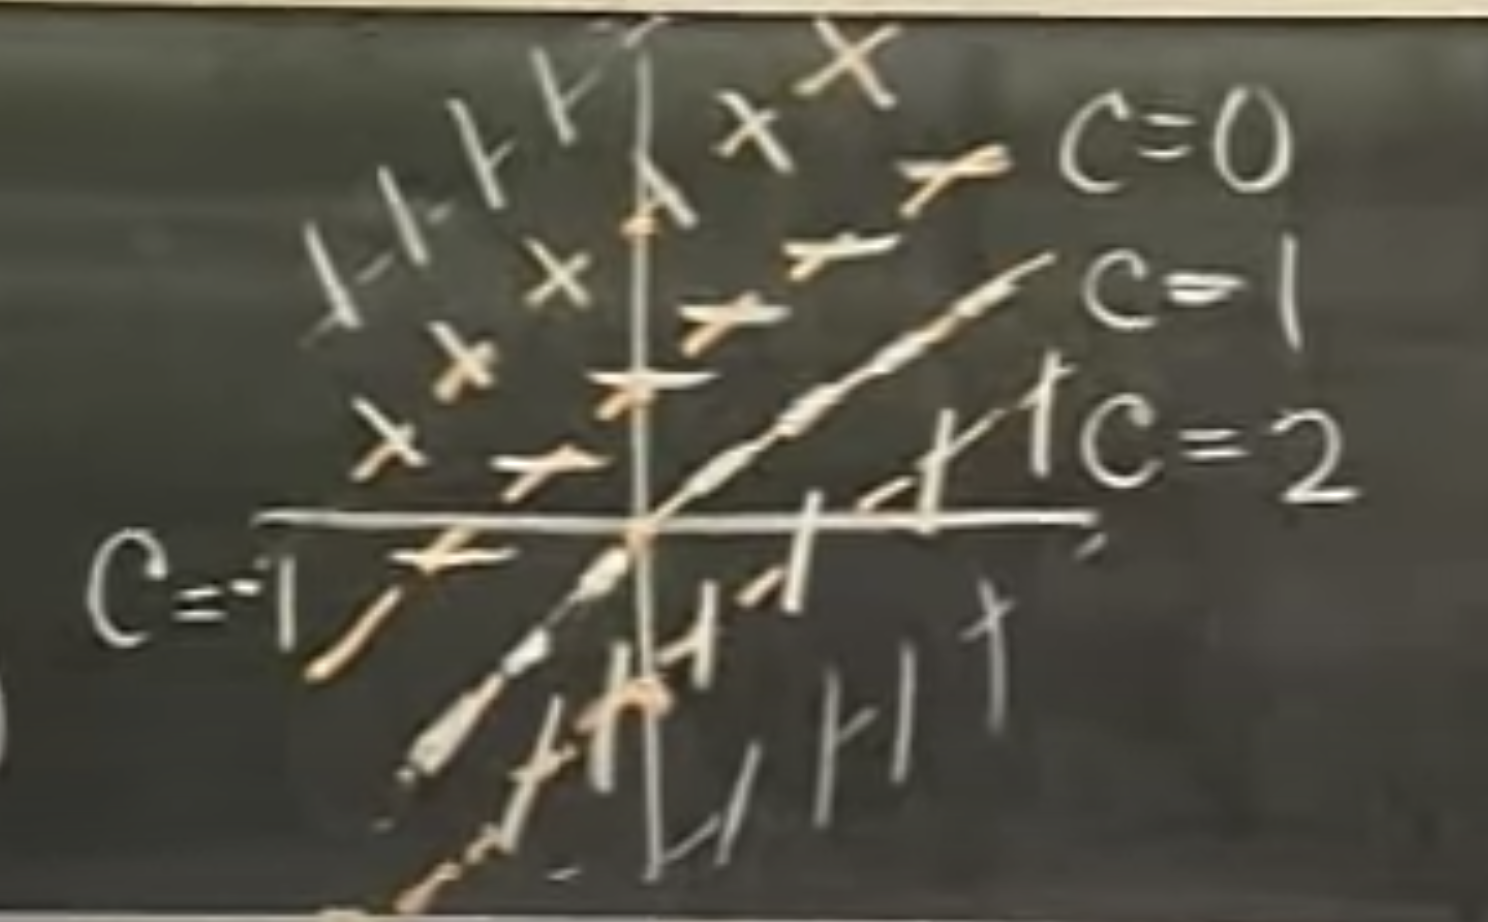
\includegraphics[scale=0.3]{./images/lecture_1_figure_2.png}
    \caption{Direction Field of $y' = 1 + x - y$ with the line elements}
\end{figure}

We can see the the line with $c = 1$ is both an Isocline and an Integral Curve.
The other Integral Curves will approch that line forever.
There is a corridor around the line  $c = 1$ where every point's line element goes towards the central line 
and if any curve enters there it will converge towards the central line.

Thus, solution cannot escape.
\begin{mdframed}
{\bf Lemma : } Two Integral Curves cannot intersect at an angle.

{\bf Proof : } If two integral curve intersect at a point at an angle then their line elements are different at that point which is impossible 
because there is only one line element at a point which is determined by the direction field.        
\end{mdframed}

Now in the above example, the integral curves that enter the corridor cannot escape.
But they cannot intersect the line with $c = 1$ so they must get closer and closer to it without every touching it.

\begin{mdframed}
{\bf Lemma : } Two Integral Curves cannot be tangent.

{\bf Proof : } This is proven by the Existence and Uniqueness Theorem.
\end{mdframed}


\section{Existence and Uniqueness Theorem}

\begin{mdframed}
{\bf Theorem : } For any point $(x_0, y_0)$, $y' = f(x, y)$ has one and only one solution through the point $(x_0, y_0)$.
\end{mdframed}

Here the requirements are that $f(x, y)$ should be continuous near $(x_0, y_0)$.
This guarantees the existence of a solution.

Another requirement is that $f_y(x, y)$ should be continuous near $(x_0, y_0)$.
This guarantees the uniqueness of the solution.


{\bf Example : } Let $xy' = y - 1$.
Solving this by separation of variables we'll get,
$$ \frac{dy}{y-1} = \frac{dx}{x} 
\Rightarrow 
ln(|y-1|) = ln(|x|) + c_1 
\Rightarrow
y - 1 = \pm e^{c_1} x 
$$

This simplifies to $y = 1 + c_2x$ where $c_2 = \pm e^{c_1}$
Here, we can see that any there is a solution through any point except the points on the y-axis.
That is because writing it in the standard form, we get, $$y' = \frac{y-1}{x}$$

Here,  we can see that it is not defined on the y-axis. 
Thus, there are no solutions through the points on the y-axis except $(0, 1)$.
And there are multiple solutions through the point $(0, 1)$ because $f_y = \frac{1}{x}$ which is undefined on the $y$-axis as well.


Hence, the only places that this theorem will fail is where $f(x, y)$ is undefined.